\section{Appendix: Project Journals}
\subsection{Project Journal 1}

\begin{longtable}{|p{4cm}|p{11cm}|}
\hline
\textbf{Section} & \textbf{Details} \\
\hline
\textbf{Title of Dissertation and Brief Description} & 
Title: Predicting Cardiovascular Diseases using Machine Learning \\
& Description: This project aims to advance the prediction of heart disease through the application of machine learning algorithms, with an emphasis on integrating explainable artificial intelligence (XAI) techniques and risk stratification models. By incorporating XAI, the project seeks to enhance the interpretability of predictive models, enabling both healthcare professionals and non-specialists to better understand the underlying factors contributing to the predictions and support in accurate clinical decision-making and treatment. \\
\hline
\textbf{Communicating with Supervisor} & 
I messaged Professor Cristina expressing interest in her supervision for the dissertation and shared the research proposal. \\
& The supervisor agreed, said she found the topic interesting and updated the allocation in the project system. We agreed on a preferred time and location for our first meeting. \\
& First meeting with Professor Cristina to get started with Dissertation (In person) – 20/09/2024. \\
& We discussed the D1 approaches, and the professor explained the details about the ethics form, and project handbook \& asked me to find a dataset used in previous research papers. She suggested I start writing from the background chapter of D1 and submit a draft to her by the end of Week 4 or the start of Week 5. I presented my research done during the summer on the proposed research topic. The supervisor advised to include 5-7 research papers due to word limit constraints.  \\
\hline
\textbf{References consulted} &
I have researched on some papers found online through Google Scholar and Discovery. 
\begin{itemize}
    \item Baghdadi, N.A. et al. (2023) ‘Advanced machine learning techniques for cardiovascular disease early detection and diagnosis’, Journal of Big Data, 10(1). doi:10.1186/s40537-023-00817-1.
    
    \item Bizimana, P.C. et al. (2024) ‘Automated heart disease prediction using improved explainable learning-based technique’, Neural Computing and Applications, 36(26), pp. 16289–16318. doi:10.1007/s00521-024-09967-6.
    
    \item Careervira (2023) Machine learning for beginners: A comprehensive 2023 guide, Medium. Available at: \url{https://medium.com/@careervira.community/machine-learning-for-beginners-a-comprehensive-2023-guide-4ec02d5caab7} (Accessed: 22 September 2024).
    
    \item García-Ordás, M.T. et al. (2023) ‘Heart disease risk prediction using Deep Learning techniques with feature augmentation’, Multimedia Tools and Applications, 82(20), pp. 31759–31773. doi:10.1007/s11042-023-14817-z.
    
    \item Holdsworth, J. and Scapicchio, \& Mark (2024) What is deep learning? IBM. Available at: \url{https://www.ibm.com/topics/deep-learning} (Accessed: 22 September 2024).
    
    \item "Hospitalization for Heart Attack, Stroke, or Congestive Heart Failure among Persons with Diabetes", Special report: 2001 – 2003, New Mexico.
    
    \item Kavitha, M. et al. (2021) ‘Heart disease prediction using Hybrid Machine Learning Model’, 2021 6th International Conference on Inventive Computation Technologies (ICICT) [Preprint]. doi:10.1109/icict50816.2021.9358597.
    
    \item Krishnani, D. et al. (2019) ‘Prediction of coronary heart disease using supervised machine learning algorithms’, TENCON 2019 - 2019 IEEE Region 10 Conference (TENCON) [Preprint]. doi:10.1109/tencon.2019.8929434.
    
    \item Latha, C.B. and Jeeva, S.C. (2019) ‘Improving the accuracy of prediction of heart disease risk based on ensemble classification techniques’, Informatics in Medicine Unlocked, 16, p. 100203. doi:10.1016/j.imu.2019.100203.
\end{itemize}
\hline

\textbf{References used} & 
\begin{itemize}
    \item Mohan, S., Thirumalai, C. and Srivastava, G., 2019. Effective heart disease prediction using hybrid machine learning techniques. IEEE access, 7, pp.81542-81554. 
    \item Schlesinger, D.E. and Stultz, C.M. (2020) ‘Deep Learning for Cardiovascular Risk Stratification’, Current Treatment Options in Cardiovascular Medicine, 22(8). doi:10.1007/s11936-020-00814-0.
 \item Shah, D., Patel, S. and Bharti, S.K. (2020) ‘Heart disease prediction using Machine Learning Techniques’, SN Computer Science, 1(6). doi:10.1007/s42979-020-00365-y.
\item Sudhakar, K. and Manimekalai, D.M., 2014. Study of heart disease prediction using data mining. International journal of advanced research in computer science and software engineering, 4(1), pp.1157-1160.
    \item UCI: Heart Failure Prediction Dataset. UCI Machine Learning Repository. (Accessed: October 2024). \url{https://archive.ics.uci.edu/dataset/45/heart+disease}
    
    \item Shankar et al. (2020) Heart Disease Prediction Using CNN Algorithm.
\end{itemize}

\hline
\textbf{Tools explored/used} & 
\begin{itemize}
    \item Github
    \item Jupyter Notebook for practising data cleaning and feature selection.
    \item Overleaf LaTeX editor
    \item Anaconda Python environment.
    \item Libraries such as numpy, scikit-learn, pandas and other data mining libraries were explored.
    \item Experimented by creating a basic model that can denote 0 and 1 for predicting heart disease.
    \item Used TensorFlow library, Gradio, Shapley
    \item Experimented with sklearn.metrics and evaluation strategies such as accuracy, precision, etc.
    \item Logistic Regression and random forests
\end{itemize} \\
\hline
\textbf{Other work carried out} &
\begin{itemize}
    \item Structure of Chapters 1 and 2 is planned out.
    \item Analysis of datasets from Kaggle and other resources.
    \item Completed writing project journal 1.
    \item Made an Excel spreadsheet on relevant prior works on the topic.
    \item Explored various Python libraries available online and referred to similar implementations on GitHub.
    \item Narrowed down the literature review to 7 research papers.
    \item Wrote a rough draft for Chapter 2 Background and cited various sources using Harvard citation style.
\end{itemize} \\
\hline
\textbf{Plan for the next 2 to 3 weeks} &
\begin{itemize}
    \item Finalize the datasets, methodologies, research questions, and objectives of the project.
    \item Analyze existing literature and choose 5-7 research papers for critical analysis.
    \item Research machine learning algorithms used in prior work and identify gaps in existing literature.
    \item Inform the supervisor about the dataset, methodologies, and objectives of the project.
    \item Complete chapter 2 of D1 and submit the draft to the supervisor.
    \item Modify and refine the draft using feedback.
    \item Familiarize with deep learning and machine learning techniques.
    \item Perform data preprocessing and understand the finalized dataset.
    \item Submit the ethics approval form in the project system.
\end{itemize} \\
\hline
\textbf{Overall Reflection} &
The dissertation work is progressing well, with significant progress made in the initial stages of the project. Communication with my supervisor has been very productive and has helped me clarify the direction of the research. The project title, objectives, and a basic research proposal have been decided, and the supervisor provided valuable feedback during our first meeting, particularly in relation to structuring the dissertation and the ethical considerations involved.  
I have explored various tools, datasets, and machine learning libraries, successfully building a preliminary model for heart disease prediction. The exploration of Python libraries such as NumPy, scikit-learn, and TensorFlow has helped me gain hands-on experience in data preprocessing and model development. However, selecting the most appropriate dataset for the final project was a challenge due to the diversity of available datasets. After careful consideration to ensure the chosen dataset aligns with the project’s goals, I have narrowed it down to 3 datasets.
The literature review is coming together, with 12 research papers identified, and I have begun drafting Chapter 2 on the background, narrowing down the review to a smaller set of key papers to meet the word limit constraint. Time management has been a challenge, particularly balancing background research with hands-on technical work and other courses. However, breaking down tasks into smaller milestones, such as completing a rough draft of Chapter 2 by the end of Week 4, has helped in staying on track. 
Looking ahead, my primary focus will be on finalizing the dataset, methodologies, and research questions, as well as critically analyzing 5-7 research papers for the literature review. Ensuring that my supervisor is kept updated on the project’s progress and incorporating feedback promptly will also be key to refining the work. The project will be fruitful through continued research and structured planning.
 \\
\hline
\caption{Project Journal 1 - Week 4}
\end{longtable}
\label{tab:journal1_dissertation_communication}
\vspace{5cm}

\subsection{Project Journal 2}
\begin{longtable}{|p{4cm}|p{11cm}|}
\hline
\textbf{Section} & \textbf{Details} \\
\hline
\textbf{Title of Dissertation and Brief Description} & 
Title: Predicting Cardiovascular Diseases using Machine Learning \\
& Description: This project aims to advance the prediction of heart disease through the application of machine learning algorithms, with an emphasis on integrating explainable artificial intelligence (XAI) techniques and risk stratification models. By incorporating XAI, the project seeks to enhance the interpretability of predictive models, enabling both healthcare professionals and non-specialists to better understand the underlying factors contributing to the predictions and support in accurate clinical decision-making and treatment.  \\ 
& Description (Updated) This project aims to advance the prediction of heart disease through the application of machine learning algorithms, and deep learning techniques with an emphasis on integrating explainable artificial intelligence (XAI) techniques and risk stratification models. By incorporating XAI, the project seeks to enhance the interpretability of predictive models, enabling both healthcare professionals and non-specialists to better understand the underlying factors contributing to the predictions and support in accurate clinical decision-making and treatment.\\
\hline
\textbf{Communicating with Supervisor} & 
I messaged Professor Cristina about the Ethics form submission and the Supervisor agreed to an online meeting where she guided me with the submissions. 
After I submitted the Ethics form, the supervisor approved it.
 Expressed interest in exploring both machine learning techniques and deep learning. The supervisor encouraged me to do it provided it doesn’t complicate the dissertation, owing to other courses and integration of explainable AI.
I informed the supervisor that I’ll be submitting a draft of some chapters towards the end of October. \\
\hline
\textbf{References consulted} &
New references were consulted between Week 4 to Week 7.

\begin{itemize}
    \item Tsao, C.W. et al. (2023) 'Heart Disease and Stroke Statistics—2023 Update: A Report From the American Heart Association,' Circulation, 147(8). \url{https://doi.org/10.1161/cir.0000000000001123}. (Tsao et al., 2023)
    
    \item Heart Disease Facts (2024). \url{https://www.cdc.gov/heart-disease/data-research/facts-stats/index.html}.
    
    \item World Health Organization: WHO (2019) Cardiovascular diseases. \url{https://www.who.int/health-topics/cardiovascular-diseases#tab=tab_1} (Accessed: 11 October, 2024)

\end{itemize}

\hline
\textbf{Tools explored/used} & 
\begin{itemize}
    \item Github
    \item Jupyter Notebook for practicing data cleaning and feature selection.
    \item Overleaf LaTeX editor
    \item Anaconda Python environment.
    \item Libraries such as numpy, scikit-learn, pandas and other data mining libraries were explored.
    \item Experimented by creating a basic model that can denote 0 and 1 for predicting heart disease.
    \item Used TensorFlow library, Gradio, Shapley
    \item Experimented with sklearn.metrics and evaluation strategies such as accuracy, precision, etc.
    \item Logistic Regression and random forests
\end{itemize} \\
\hline
\textbf{Other work carried out} &
\begin{itemize}
    \item Submitted the Ethics form for approval
    \item Combined datasets from UCI and integrated them into a single Excel file
    \item Expressed interest in exploring deep learning models.
    \item Made an Excel spreadsheet on relevant prior works on the topic.
    \item Completed writing project journal 2. 
    \item Explored various python libraries available online and referred to similar implementations on GitHub. 
    \item Refined Chapters 1 and 2.
     \item Drafted Chapters 3,4 and 5.
 \item Completed risk analysis and the Gantt Chart for project management which are included in the Appendix.
 \item Formatted the report in the latex editor

\end{itemize} \\
\hline
\textbf{Plan for the next 2 to 3 weeks} &
\begin{itemize}
\item Complete chapters 3,4 and 5 of D1 and submit the draft to the supervisor for reviewing by the end of week 8.
\item Complete the draft of the Requirements Analysis and Methodology chapter.
\item Refine Functional and Non-Functional Requirements 
\item Connect them with the objectives using a traceability matrix.
\item Formulate research questions for the project.
\item Modify and refine the draft using feedback provided by the supervisor.
\item Familiarize with deep learning and machine learning techniques.
\item Perform data preprocessing and understand the finalized dataset. 
\item Finally, draft other sections of D1.
\item Draft the PLES section.
\item Add references. 
\item Feedback Iterations: After getting feedback from the supervisor for the draft, add her insights and refine the report accordingly. 

\end{itemize} \\
\hline
\textbf{Overall Reflection} &
The deliverable 1 is progressing well. I have completed chapters 1 and 2 and refined them. Chapters 3,4 and 5 are drafted and will be refined for clarity. I converted the report from Word format to latex for better presentation. The appendix section has been drafted. It has been a little challenging with all other courses having submissions within the same week, but with a better time management plan, the D1 will successfully be completed.
 \\
\hline
\caption{ Project Journal 2 - Week 7}
\end{longtable}


\subsection{Project Journal 3}
\begin{longtable}{|p{4cm}|p{11cm}|}
\hline
\textbf{Section} & \textbf{Details} \\
\hline
\textbf{Title of Dissertation and Brief Description} & 
Title: Predicting Cardiovascular Diseases using Machine Learning \\
& Description: This project aims to advance the prediction of heart disease through the application of machine learning algorithms, and deep learning techniques with an emphasis on integrating explainable artificial intelligence (XAI) techniques and risk stratification models. By incorporating XAI, the project seeks to enhance the interpretability of predictive models, enabling both healthcare professionals and non-specialists to better understand the underlying factors contributing to the predictions and support in accurate clinical decision-making and treatment.\\
\hline
\textbf{Communicating with Supervisor} & 
I submitted drafts of Chapters 1,2,3 and 5 along with appendices Dr Cristina. 
Feedback from the Supervisor: She appreciated my works and asked for some minor modifications such as adding the word Chapter in front of Chapter headings. She also asked me to modify some functional requirements and remove the validation section. I have completed those modifications. 
I will be submitting the final draft for review on the 12th or 13th of November 2024. My ethics form got approved and I plan to submit the D1 on Canvas a few days in advance to allow time for any last-minute adjustments.
 \\
\hline
\textbf{References consulted} &
New references were consulted from Week 7 onwards.

\begin{itemize}
    \item Multi Disease Prediction System using Random Forest Algorithm in Healthcare System.
    \item A Systematic Review of Artificial Intelligence Models for Time-to-Event Outcome Applied in Cardiovascular Disease Risk Prediction.  
    \item Artificial intelligence in the risk prediction models of cardiovascular disease and development of an independent validation screening tool: a systematic review. 
    \item Predicting Heart Attack through Explainable Artificial Intelligence. 
    \item Automated heart disease prediction using improved explainable learning-based technique. 
    \item Optimized Ensemble Learning Approach with Explainable AI for Improved Heart Disease Prediction.
    \item \url{https://link.springer.com/article/10.1007/s00521-024-09967-6} 
    \item \url{https://www.iraj.in/journal/journal_file/journal_pdf/6-71-140490825388-92.pdf}    
    \item \url{https://ieeexplore.ieee.org/abstract/document/8971374}    
    \item \url{https://ieeexplore.ieee.org/stamp/stamp.jsp?tp=&arnumber=6164626}   
    \item \url{https://link.springer.com/article/10.1007/s11042-022-14305-w}  
    \item \url{https://link.springer.com/article/10.1007/s00500-022-07788-0?fromPaywallRec=true}
\end{itemize}

\hline
\textbf{Tools explored/used} & 
\begin{itemize}
\item Data visualization tools 
\item Python libraries such as numpy, scikit-learn, pandas
\item Experimented by creating a basic model that can denote 0 and 1 for predicting heart disease.
\item Pytorch
\item Implementation of Decision trees, random forests, 
\item Deep learning models like perceptron and fully connected neural networks 
Other work carried out	
\item Submitted the draft of Chapters 1,2,3 and 5 to the supervisor.
\item Incorporated supervisor’s feedback to the report. 
\item Explored various python libraries available online and referred to similar implementations on GitHub. 
\item Finalized Chapters 1 and 2.
\item Completed Chapters 3,4 and 5- the draft of the Requirements Analysis and Methodology chapter.
\item Completed risk analysis and the Gantt Chart for project management which are included in the Appendix
\item Completed the PLES section
\item Completed grammar, and spelling checks.
\item Completed plagiarism check and ensured all sources consulted are referenced, 
\item Formatted the report and enhanced its structure.
\item Ensured the main body doesn’t exceed 20 pages.
\item Research on evaluation strategies for assessing model performance.
\item Read through other D1 provided on Canvas for inspiration.

\end{itemize} \\
\hline
\textbf{Other work carried out} &
\begin{itemize}
\item Submit the final draft with all chapters for review on the 12th or 13th of November 2024 ensuring adequate time is left for refinements.
\item Feedback Iterations: After getting feedback from the supervisor for the draft, incorporate her insights and refine the report accordingly. 
\item Create a folder that contains D1 report, Standard Declaration of Authorship form and project journals.
\item Once the supervisor’s feedback is added and finalized, submit the final version of D1 on Canvas.  
\item Familiarize with deep learning and machine learning techniques.
\item Perform data preprocessing and understand the finalized dataset. 


\end{itemize} \\
\hline
\textbf{Plan for the next 2 to 3 weeks} &
\begin{itemize}
\item Complete chapters 3,4 and 5 of D1 and submit the draft to the supervisor for reviewing by the end of week 8.
\item Complete the draft of the Requirements Analysis and Methodology chapter.
\item Refine Functional and Non-Functional Requirements 
\item Connect them with the objectives using a traceability matrix.
\item Formulate research questions for the project.
\item Modify and refine the draft using feedback provided by the supervisor.
\item Familiarize with deep learning and machine learning techniques.
\item Perform data preprocessing and understand the finalized dataset. 
\item Finally, draft other sections of D1.
\item Draft the PLES section.
\item Add references. 
\item Feedback Iterations: After getting feedback from the supervisor for the draft, add her insights and refine the report accordingly. 

\end{itemize} \\
\hline
\textbf{Overall Reflection} &
Overall Reflection	Deliverable 1 is almost completed. I have completed the main body of D1- Chapters 1,2,3,4 and 5 and I’m refining them further. The appendix section is complete with the PLES section, project management and project journals. It has been a little challenging with all other courses having submissions within the same week. But I’m on track. I will be having another detailed review of the report to ensure it adheres to the guidelines given in the project handbook.
I have simultaneously gained knowledge of the technical aspects of the project. I have familiarized myself with the data preprocessing techniques and various machine learning models. I have also researched the evaluation strategies to assess how the model is performing. I will refine my report and submit it to my supervisor on 12th or 13th November for her feedback.  I feel so happy. Completion of the main body of D1 marks an important milestone in the Dissertation. I’m grateful for Dr Cristina and her valuable feedback throughout this journey. 

\hline
\caption{ Project Journal 3 - Week 10}
\end{longtable}
\label{tab:journal1_dissertation_communication}

\begin{figure}[htbp]
    \centering
    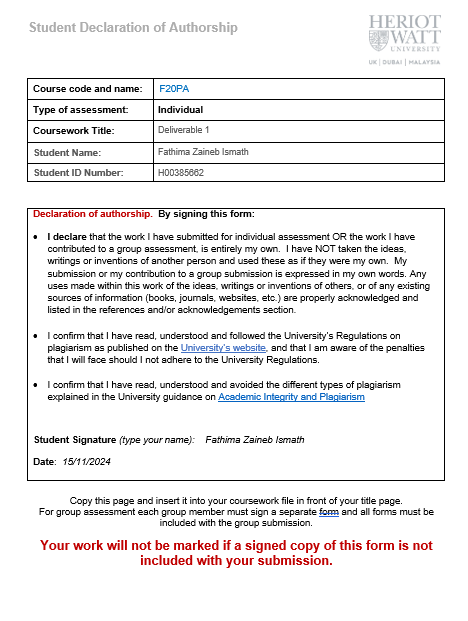
\includegraphics[width=0.8\textwidth]{appendices/images/declaration.PNG}
    \caption{Standard Declaration of Authorship}
    \label{fig:declaration_form}
\end{figure}
